%% Theorie.tex
%%
%\usepackage[ngerman]{babel}
%% ==============
\chapter{Experimentelle Grundlagen}
\label{ch:experiment}
%% ==============

{\bibliographystyle{babalpha-fl}}	% german style

Zur Untersuchung der theoretischen Vorhersagen des Standardmodells, werden weltweit Experimente durchgef\"uhrt. In Kapitel \ref{ch:experiment} werden die experimentellen Grundlagen anhand des Compact-Muon-Solenoid-Experiment (CMS, Abschnitt \ref{ch:Experiment:sec:CMS}) am Large-Hadron-Collider (LHC, Abschnitt \ref{ch:Experiment:sec:LHC}) des CERN vorgestellt. Anschlie\ss end wird der Ablauf einer Hochenergiephysik-Analyse am Beispiel der \ttH-Analyse vorgestellt.

%% ===========================
\section{Der Large Hadron Collider (LHC)}
\label{ch:Experiment:sec:LHC}
%% ===========================

Der Large-Hadron-Collider (LHC) ist ein Teilchenbeschleuniger der Europ\"aischen Organisation f\"ur Kernforschung (CERN). Er befindet sich in einem 26,7 km langen Tunnel im Grenzgebiet zwischen Frankreich und der Schweiz bei Genf zwischen 45 m und 170 m unter der Erdoberfl\"ache. Es ist der zur Zeit leistungsst\"arkste Teilchenbeschleuniger der Welt.\\
Der LHC kann mit Protonen oder Bleiionen betrieben werden. Wenn Protonen genutzt werden, durchlaufen diese zun\"achst in einer Reihe von Vorbeschleunigern in denen sie pr\"apariert werden. Als erstes wird Wasserstoffgas ionisiert. Die so entstehenden Protonen werden im LINAC2, einem Linearbeschleuniger in B\"undeln (bunches) mit je $1,1\cdot 10^{11}$ Protonen auf 50 MeV beschleunigt \cite{O'Luanaigh:1997427}. Anschlie\ss end werden die Protonenbunches im Proton-Synchrotron-Booster (PSB), im Proton-Synchroton (PS) und im Super-Proton-Synchrotron (SPS) erst auf 1,4 GeV, dann auf 25 GeV und schlie\ss lich auf 450 GeV beschleunigt \cite{O'Luanaigh:1997193}. Im LHC selbst werden in zwei Strahlr\"ohren jeweils maximal 2808 bunches in entgegengesetzte Richtungen auf maximal 7 TeV beschleunigt \cite{Lefevre:1165534}. Die Protonen werden an bestimmten Punkten zur Kollision gebracht. \\
Es gibt sieben Experimente die die bei den Kollisionen entstehenden Teilchen untersuchen. Diese Experimente werden von Kollaborationen von Wissenschaftlern aus aller Welt durchgef\"uhrt. Die beiden gr\"o\ss ten sind ATLAS und CMS, die mit ihren universellen Teilchendetektoren alle entstehenden Kollisionsprodukte untersuchen k\"onnen, w\"ahrend bei dem Schwerionen-Experiment ALICE (A Large Ion Collider Experiment) und dem Large-Hadron-Collider-beauty-Experiment (LHC-B) spezifische Ph\"anomene untersucht werden. ALICE wurde entwickelt um durch Kollisionen von Bleiionen ein Quark-Gluon-Plasma zu erzeugen, was den Bedingungen kurz nach dem Urknall entspricht. LHC-B untersucht Unterschiede zwischen Materie und Antimaterie mithilfe von b-Quarks. Die kleineren Experimente sind TOTEM (Total, elastic and diffractive cross-section measurement) und LHCf (Large Hadron Collider forward), die beide "vorw\"arts" gestreute Ereignisse, also Ereignisse mit sehr kleinem Streuwinkel untersuchen, sowie MoEDAL (Monopole and Exotics Detector at the LHC), das nach magnetischen Monopolen sucht. \cite{O'Luanaigh:1997374, O'Luanaigh:1997265, O'Luanaigh:1997262, O'Luanaigh:1997259, O'Luanaigh:1997373, O'Luanaigh:1997527}\\
In Abbildung \ref{fig:LHC} ist der schematische Aufbau des LHC mit den Experimenten CMS, Atlas, LHC-B und ALICE abgebildet. Die Vorbeschleuniger sind dabei au\ss er dem SPS nicht ber\"ucksichtigt.

\begin{figure}[hhh]
 \begin{center}
   \includegraphics[width=0.8\textwidth]{graphics/LHC_experiments.jpg}
   \parbox[b]{12cm}{
     \caption[Large-Hadron-Collider]
             {\label{fig:LHC} \it\!Der LHC mit den vier Hauptexperimenten und dem Super-Proton-Synchrotron, \cite{Team:40525}}
   }
 \end{center}
\end{figure}

%% ===========================
\section{Der Compact-Muon-Solenoid-Detektor (CMS)}
\label{ch:Experiment:sec:CMS}
%% ===========================

Der Compact-Muon-Solenoid (CMS) ist einer der beiden universellen Teilchendetektoren am LHC. Sein Aufbau ist in Abbildung \ref{fig:cms_sectional} zu sehen. Am CMS-Experiment arbeiten zurzeit etwa 4300 Personen mit \cite{cms_people}. Der Detektor ist mit etwa \num{14000} Tonnen und einem Durchmesser von \num{15} Metern auf circa \num{28,7} Meter L\"ange recht kompakt gebaut. Dies war m\"oglich, da die einzelnen Teile \"uberirdisch gefertigt wurden und erst in der Kaverne ungef\"ahr \num{100} Meter unter der Erde zusammengebaut wurden.\\
\begin{figure}[hhh]
 \begin{center}
   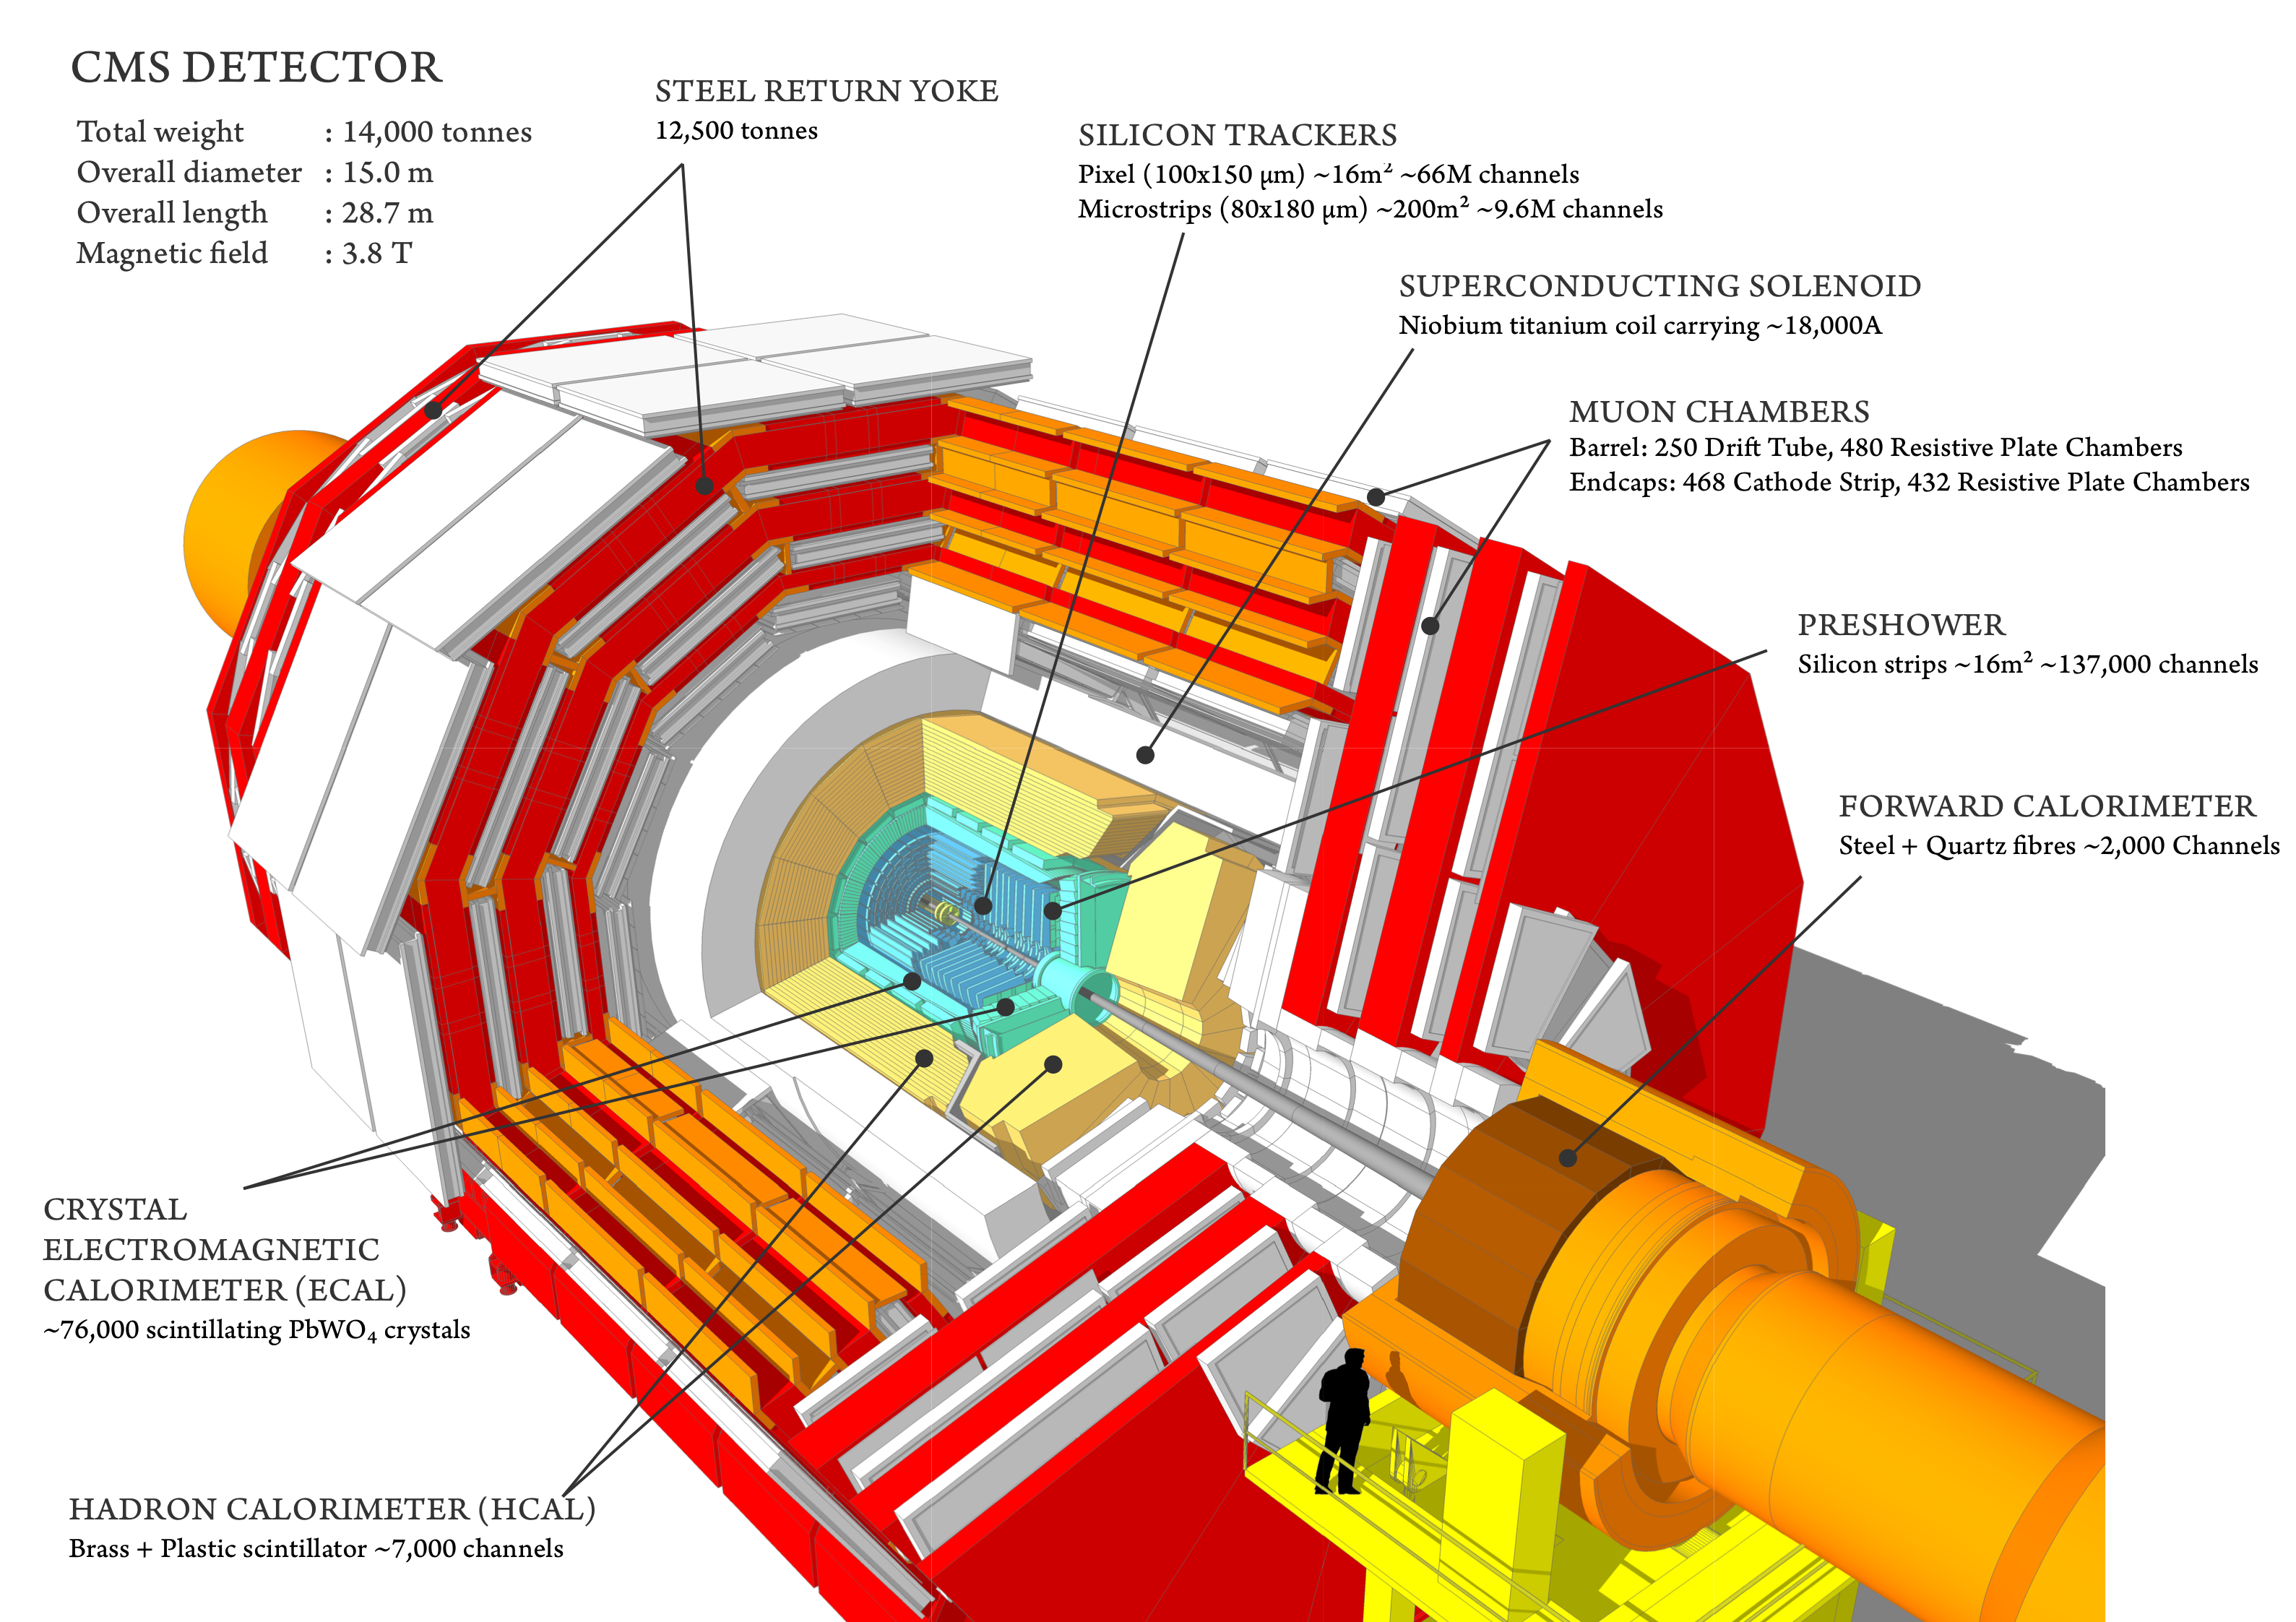
\includegraphics[width=\textwidth]{graphics/cms_sectional.png}
   \parbox[b]{12cm}{
     \caption[CMS-Detektor]
             {\label{fig:cms_sectional} \it\!Der CMS-Detektorv im Querschnitt, \cite{cms_sectional}}
   }
 \end{center}
\end{figure}

Der CMS-Detektor ist kein einzelner Detektor, sondern besteht aus mehereren Detektoren, die in zylinderf\"ormigen Lagen, \"ahnlich einer Zwiebel, \"ubereinandergeschichtet sind. Herz- und namensgebendes St\"uck ist der gro\ss e Magnet (solenoid), der ein bis zu \num{4} Tesla starkes homogenes Magnetfeld erzeugt, durch das geladene Teilchen abgelenkt werden, um ihren Impuls bestimmen zu k\"onnen. Die innerste Lage bilden der Spurdetektor. Er besteht aus Silizium-Pixeldetektoren und Silizium-Streifendetektoren. Sie bestimmen die Spuren der bei der Kollision erzeugten Teilchen. Als n\"achste Schicht ist ein elektromagnetisches Kalorimeter (ECAL) aus Bleiwolframat-Kristallen (PbWO$_4$) eingebaut, mit dem Elektronen, Positronen und Photonen nachgewiesen und \"uber die Energie des elektromagnetischen Schauers auch ihre Energie bestimmt werden kann. Das ECAL wird umschlossen von einem hadronischen Kalorimeter (HCAL), das zur Identifizierung und Energiemessung der Hadronen verwendet wird. An diese Lage schlie\ss t sich die Magnetspule an. Au\ss erhalb des Magneten befinden sich das eiserne R\"uckf\"uhrjoch, das von Myonenkammern zum Nachweis von Myonen durchzogen ist.\\

\begin{figure}[hhh]
 \begin{center}
   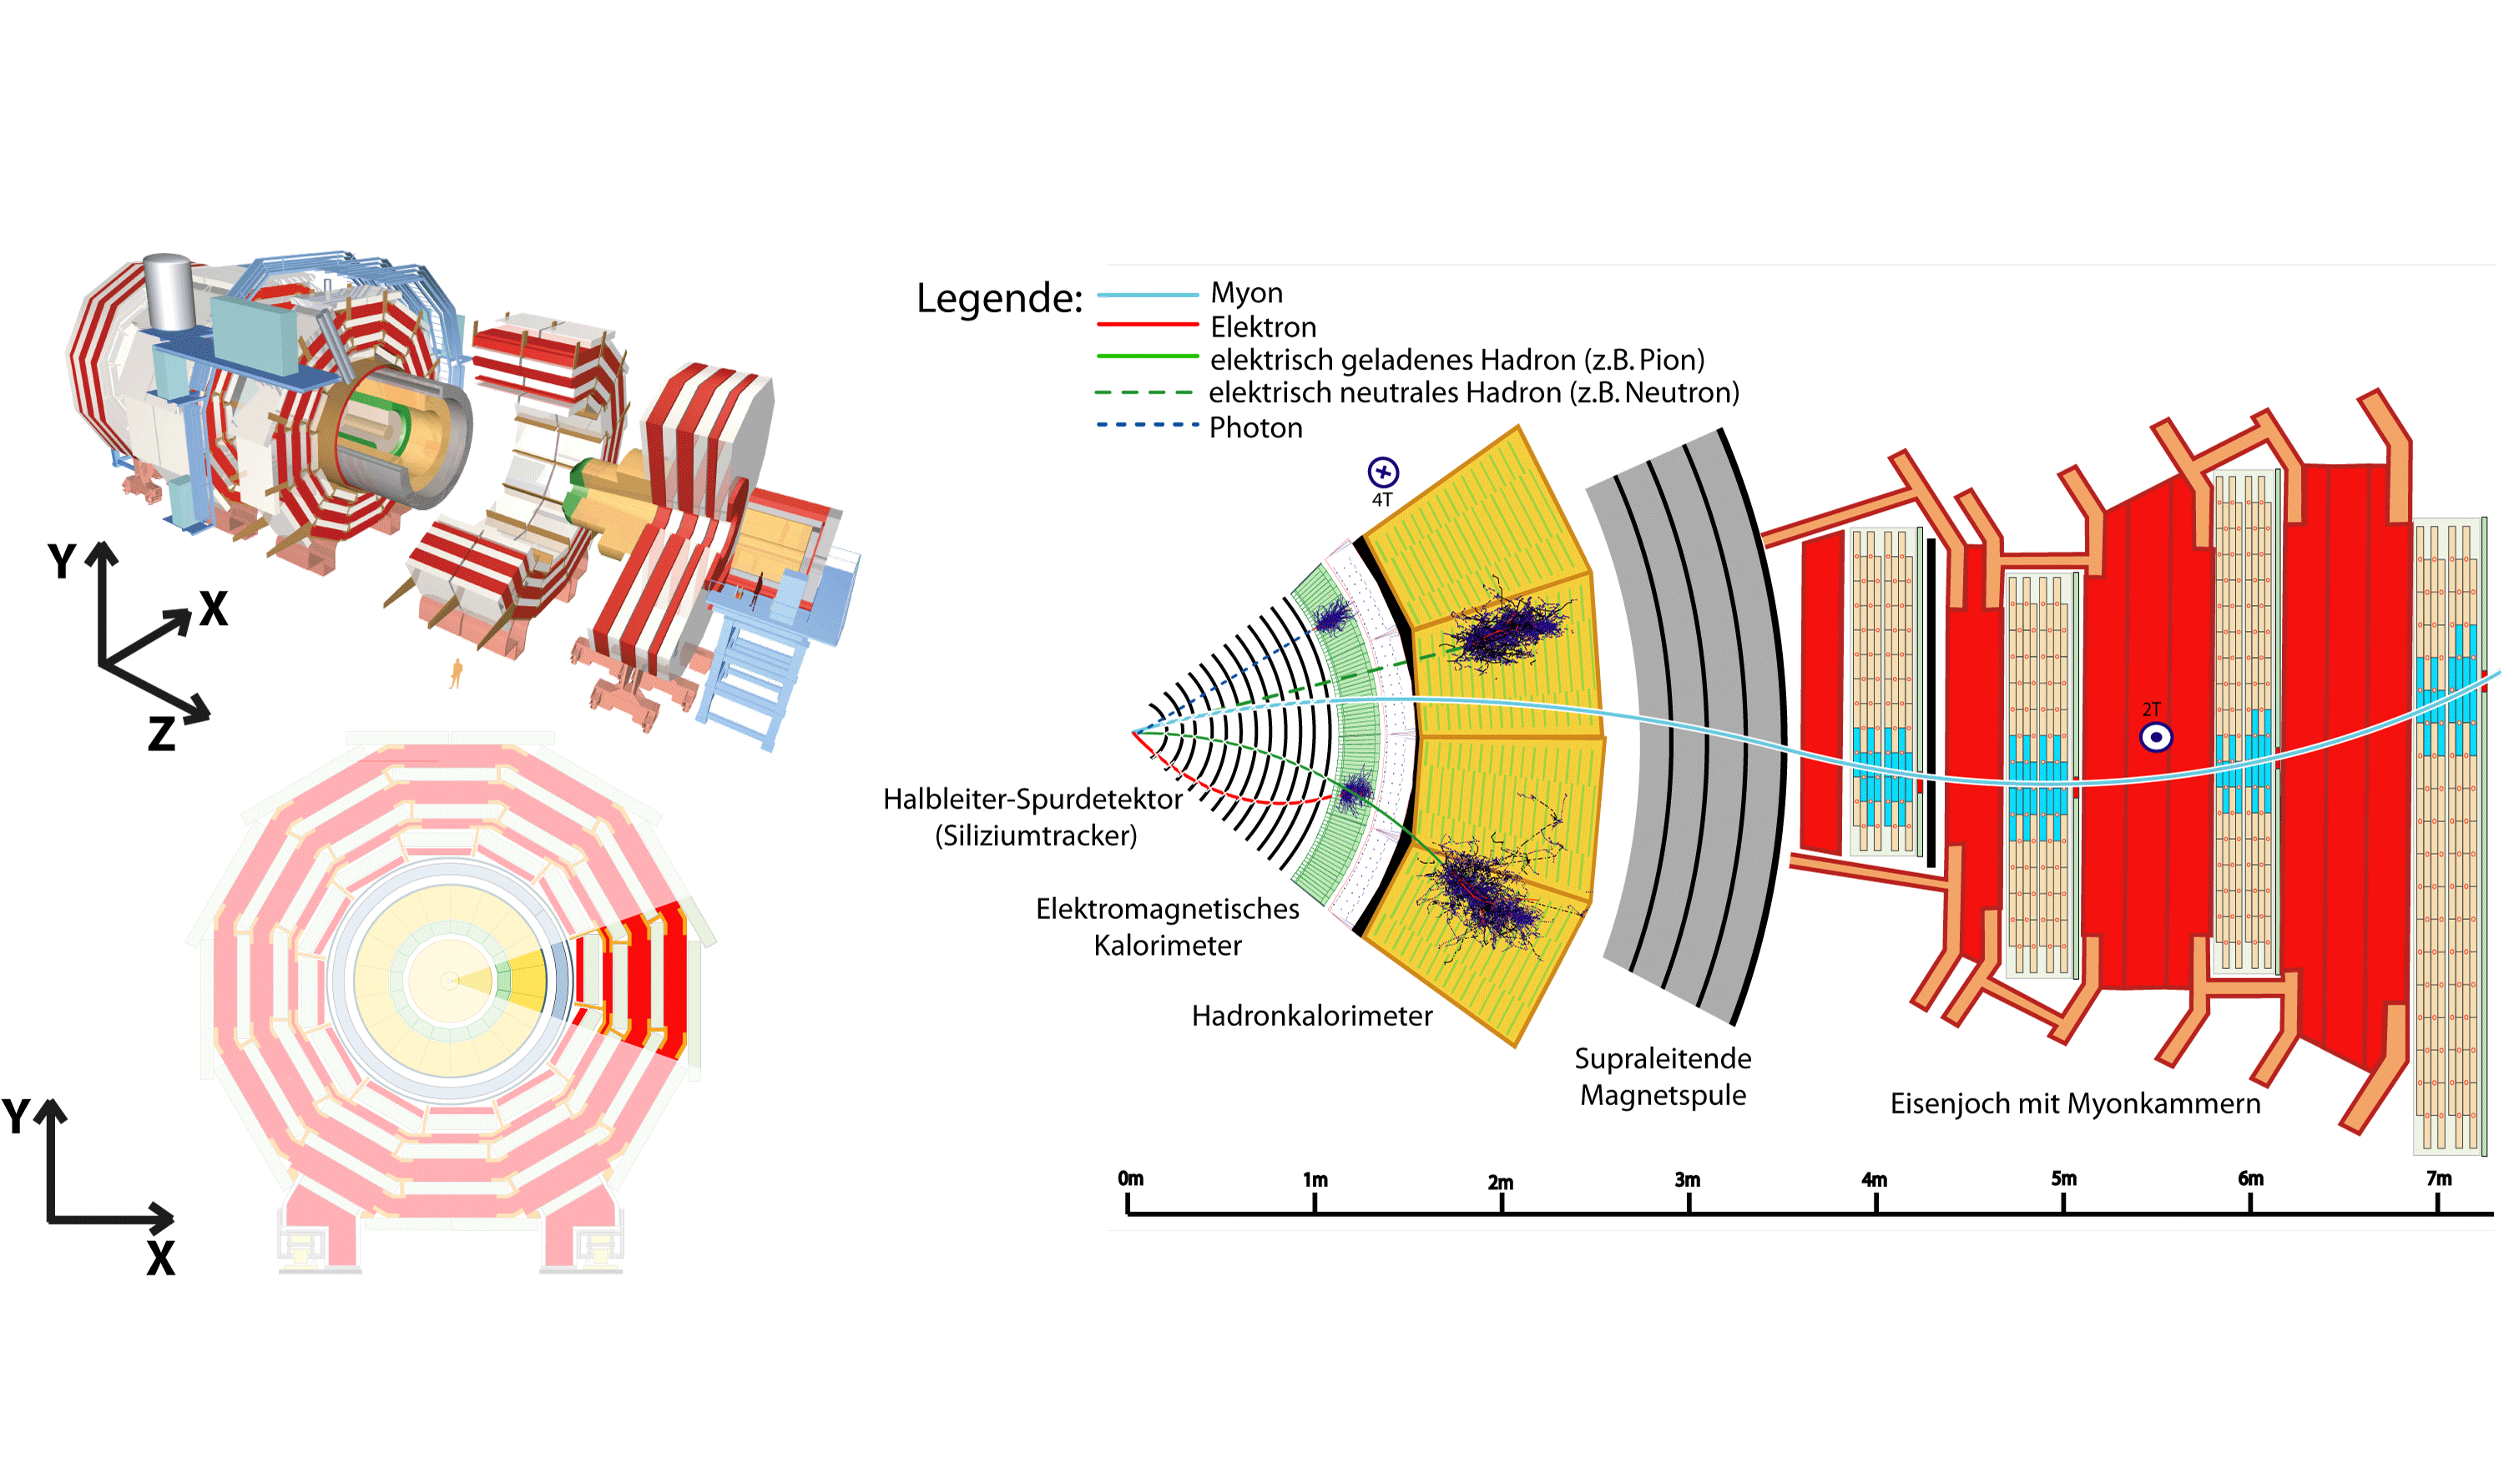
\includegraphics[width=\textwidth]{graphics/cms_slice.png}
   \parbox[b]{12cm}{
     \caption[CMS-Detektor]
             {\label{fig:cms_slice} \it\!Ausschnitt des CMS-Detektors mit verschiedenen Teilchenbahnen, \cite{cms_slice}}
   }
 \end{center}
\end{figure}

In Abbildung \ref{fig:cms_slice} ist nochmals ein Ausschnitt des CMS-Detektors mit den Trajektorien der einzelnen Teilchen abgebildet. Im linken oberen Bereich ist der komplette Detektor mit auseinandergefahrenen Segmenten zu sehen. Darunter ist der Querschnitt gezeigt, die hervorgehobene Sektion ist rechts daneben gr\"o\ss er dargestellt. Man erkennt die einzelnen Schichten des Detektors. Die rote Linie zeigt beispielhaft das Verhalten eines Elektrons, das w\"ahrend es den Spurdetektor durchl\"auft vom Magnetfeld abgelenkt wird und schlie\ss lich im elektromagnetischen Kalorimeter einen Schauer erzeugt wodurch es detektiert werden kann. In gr\"un sind die Trajektorien von Hadronen gezeigt. Die gestrichelte Linie entspricht einem ungeladen, die durchgezogene einem positiv geladenen. Beide erzeugen im Hadronenkalorimeter Schauer. Wie ein ungeladenes Hadron wird auch ein Photon (blau gestrichelte Linie) nicht vom Magnetfeld abgelenkt, allerdings erzeugt es bereits im ECAL einen Schauer. Ein Anti-Myon (blaue durchgezogene Linie) interagiert nicht mit den inneren Schichten des Detektors und wird daher erst in den Myonenkammern detektiert.

%% ===========================
\section{\ttH-Analyse}
\label{ch:Experiment:sec:ttH}
%% ===========================

Der kleine Wirkungsquerschnitt und die vielen Hintergrundprozesse machen eine Messung der \ttH-Produktionsrate sehr anspruchsvoll. Darum ist es essenziell, in jedem Bereich der Analyse m\"oglichst nahe am Optimum zu sein. Im folgenden soll die \ttH-Analyse am CMS-Experiment kurz erl\"autert werden. Einige der verwendeten und dar\"uberhinausf\"uhrende Informationen finden sich in \cite{Khachatryan:2014qaa}.

Der \ttH-Analyse liegen durch das Standardmodell motivierte Berechnungen zugrunde. Anhand der verschiedenen vorhergesagten Endzust\"ande werden die einzelnen Produktionskan\"ale in verschiedene Kategorien unterteilt, die sich in wesentlichen Punkten unterscheiden. Die experimentell gemessenen Rohdaten werden zun\"achst weiter verarbeitet. Es wird versucht anhand der Endzust\"ande auf Zwischenschritte der Teilchenkollisionen zur\"uckzuschlie\ss en. Dies ist n\"otig, da insbesondere Top-Quarks eine zu hohe Masse haben, um mit anderen Quarks Hadronen zu bilden, sondern viel schneller wieder zerfallen. Mithilfe von Teilchenphysikalischen Methoden wie dem Erkennen von Bottom-Quarks (b-tagging) auf die hier nicht n\"aher eingegangen wird, werden f\"ur die verschiedenen Kollisionsprodukte physikalische Eigenschaften bestimmt. Diese k\"onnen beispielsweise Transversalimpuls oder rekonstruierte Teilchenmasse sein, aber teilweise auch konstruierte Gr\"o\ss en ohne Physikalische Motivation. Diese Eigenschaften sind Variablen, die mithilfe von statistischen Analysemethoden unterschieden werden sollen.\\
Um die gesuchten Ereignisse aus den anderen Produkten der Teilchenkollissionen herauszufiltern, werden Multivariate Analysemethoden (Kapitel \ref{ch:algorithmen}) verwendet.\\
Dazu ist es entscheident, die Struktur der aufgenommenen Daten bereits zu kennen. Aus diesem Grund werden mithilfe von Monte-Carlo-Methoden, die auf die theoretischen Werte sowie Wissen \"uber das Detektorverhalten basieren, Simulationsdaten erstellt. Die gew\"unschten und gesuchten Ereignisse sind in den Simulationsdaten daher ebenso wie die unerw\"unschten Untergrunddaten bekannt, so ist es m\"oglich Algorithmen multivariater Methoden darauf anzuwenden. Dadurch lernen die Algorithmen selbst\"andig (mechine learning) verschiedenartige Daten zu Unterscheiden. Damit wird versucht aus den experimentell gemessenen Daten die gesuchten \ttH-Signale zu extrahieren.\\
Zuletzt werden die verschiedenen Kategorien wieder zusammengefasst.
